\chapter{Benchmark}

\section{Queries}

Zur Durchf�hrung des Benchmarks wurde ein Transaktionsmix von sechs Queries und zugeh�riger Aufrufh�ufigkeit betrachtet:

\begin{itemize}
 
  \item Q1 - Sitzplatzverteilung Bundestag mit Kuchendiagramm (H�ufigkeit: 25\%)
  \item Q2 - Liste der Abgeordneten (H�ufigkeit: 10\%)
  \item Q3 - Detailergebnisse eines beliebigen Wahlkreises (H�ufigkeit: 25\%)
  \item Q4 - Wahlkreissieger mit eingef�rbter Deutschlandkarte (H�ufigkeit: 10\%)
  \item Q5 - �berhangsmandate (H�ufigkeit: 10\%)
  \item Q6 - Knappste Sieger und knappste Verlierer (H�ufigkeit: 20\%)
 
\end{itemize}

Q3 arbeitet auf Wahlkreis-aggregierten Stimmen. Das hei�t f�r jeden Wahlkreis befindet sich f�r alle darin angetretenen Kandidaten und Parteien
bereits die Summe der abgegebenen Erst- bzw. Zweitstimmen als Eintrag in einer Datenbanktabelle.

Um dennoch die Performance des Systems auf Einzelstimmen zu testen, betrachten wir gesondert ein Query Q7, das das gleiche berechnet wie Q3, dem
allerdings Einzelstimmen f�r die Berechnung zugrunde liegen: 

\begin{itemize}

  \item Q7 - Detailergebnisse eines beliebigen Wahlkreises (Einzelstimmen)
 
\end{itemize}

Da Q7 �ber 62 Millionen Tupel aggregieren muss, wurden f�r den Benchmark aus Laufzeitgr�nden nur die Stimmen der Wahlkreise 213 - 217 in die
Datenbank geladen. 

\section{Messverfahren und Ziele}

 Neben der Laufzeit der Queries untereinander wurde insbesondere ihre Skalierf�higkeit getestet. Au�erdem gab der Benchmark Aufschluss dar�ber
 welche tempor�re Tabellen-Strategie mehr Performanz aufweist.
 
 \subsection{Tempor�re Tabellen}
 
 Alle Quieres benutzen f�r die Berechnung von Zwischenergebnissen tempor�re Tabellen. In DB2 gibt es daf�r im Wesentlichen zwei Ans�tze:
 Das explizite Erstellen tempor�rer Tabellen mittels \texttt{CREATE GLOBAL TEMPORARY TABLE} oder die Verwendung von Tables, die mittels dem 
 SQL-Befehl \texttt{WITH} erstellt wurden. Die wesentlichen Unterschiede der beiden Methoden liegen in ihrer Lebensdauer \footnote{DB2 Temporary Tables: 
 \url{http://www.cs.newpaltz.edu/~pletcha/DB/db2_TempTables.html}}.
 Um die Performanz der beiden Methoden zu testen wurde der Benchmark f�r Q1-Q5 einmal unter Verwendung von \texttt{GLOBAL TEMPORARY TABLE}s und
 einmal mittels \texttt{WITH} durchgef�hrt.
 
 \subsection{Testen der Skalierf�higkeit}

 Die Messung wurde mit 1, 2, 5, 7 und 10 parallel aktiven simulierten Browsern durchgef�hrt. F�r die Queries Q1 - Q6 wurde der Benchmark
 einmal mit zwei Sekunden und einmal mit vier Sekunden Wartezeit zwischen den Queries durchgef�hrt.
 
 \subsection{Technisches}
 
 Alle simulierten Browser sind in Java geschrieben und stellten alle Anfragen nach ihrer H�ufigkeit in zuf�lliger Reihenfolge an einen 
 lokalen Tomcat-Server.
 Auf dem Server lief ebenfalls Java-Code der die entsprechenden SQL-Statements generierte und an einen lokalen DB2-Server weiterleitete. 
 Aus der DB2-Antwort wurde dann mittels Servlets eine HTML-Seite generiert und an den simulierten Browser gesendet, der die Zeit
 zwischen Anfrage und Antwort stoppte. Der Benchmark wurde auf einem Intel Core 2 Duo mit 1.50 GHz und 2.00 GB RAM durchgef�hrt. 
 
 \newpage
 \section{Ergebnisse}
 
 Folgende Diagramme zeigen die Performance der einzelnen Quieres unter steigender Anzahl von parallelen Zugriffen.
 Auf der x-Achse befindet sich die Anzahl der parallel aktiven Browser und auf der
 y-Achse die dazugeh�rige durchschnittliche Server-Responsetime in Millisekunden. 
 
 \subsection{Q1 - Q6 mit 4 Sekunden Wartezeit}
 
 Das Benchmark-Ergebnis mit einer Wartezeit von jeweils \emph{vier} Sekunden pro Browser zwischen den Queries:
 
 \begin{figure}[htbp]
	\centering
		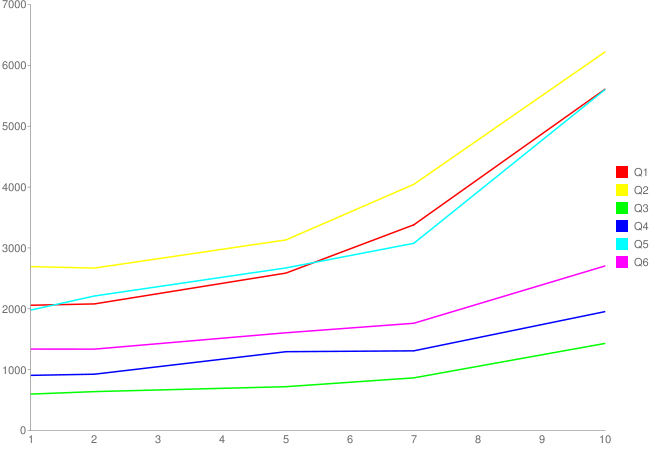
\includegraphics[width=0.85\textwidth]{figures/benchmark-4000.png}
	\caption{Durchschnittliche Response-Time bei einer Wartezeit von 4 Sekunden}
	\label{fig:benchmark-4000}
\end{figure}
 
 Man sieht dass die Berechnung von Q3 (Detailergebnisse Wahlkreis) am schnellsten ist, w�hrend die Berechnung von Q2 (Abgeordneten)
 am l�ngsten dauert.
 
 \newpage
 \subsection{Q1 - Q6 mit 2 Sekunden Wartezeit}
 
 Das Benchmark-Ergebnis mit einer reduzierten Wartezeit von jeweils \emph{zwei} Sekunden pro Browser zwischen den Queries:
 
 \begin{figure}[htbp]
	\centering
		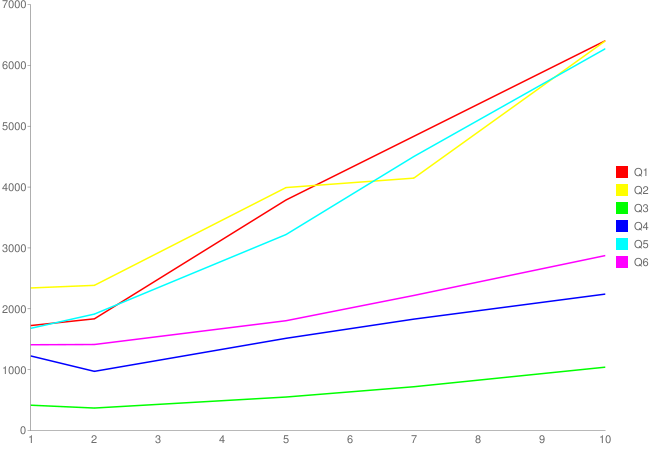
\includegraphics[width=0.85\textwidth]{figures/benchmark-2000.png}
	\caption{Durchschnittliche Response-Time bei einer Wartezeit von 2 Sekunden}
	\label{fig:benchmark-2000}
 \end{figure}
	
 Bei noch h�herer Server-Belastung ben�tigen die Queries Q1, Q2 und Q5 bei 10 parallelen Browsern schon durchschnittlich mehr als 7 Sekunden
 um zu antworten.
	
 \newpage
 \subsection{Q1 - Q6 mit 4 Sekunden Wartezeit und \texttt{WITH}-Tables}
 
 Das Benchmark-Ergebnis mit einer Wartezeit von vier Sekunden unter der Verwendung von \texttt{WITH}-Tables:
 
 \begin{figure}[htbp]
	\centering
		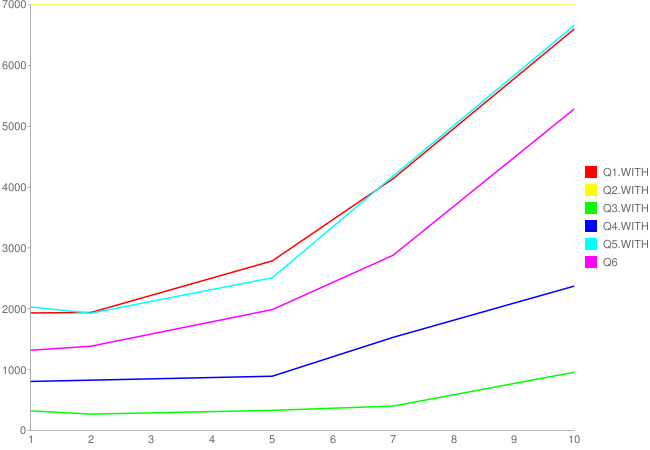
\includegraphics[width=0.85\textwidth]{figures/benchmark-WITH-4000.png}
	\caption{Durchschnittliche Response-Time bei einer Wartezeit von 4 Sekunden unter Verwendung von \texttt{WITH}-Tables}
 \end{figure}
 
 Man sieht sofort dass Q2 durch \texttt{WITH}-Tables deutlich langsamer geworden ist. Die anderen Queries sind dadurch
 im Allgemeinen etwas schneller geworden, insbesondere Q3.
 
 \newpage
 \subsection{Q1 - Q6 mit 2 Sekunden Wartezeit und \texttt{WITH}-Tables}
 
 Das Benchmark-Ergebnis mit einer Wartezeit von zwei Sekunden unter der Verwendung von \texttt{WITH}-Tables:
 
 \begin{figure}[htbp]
	\centering
		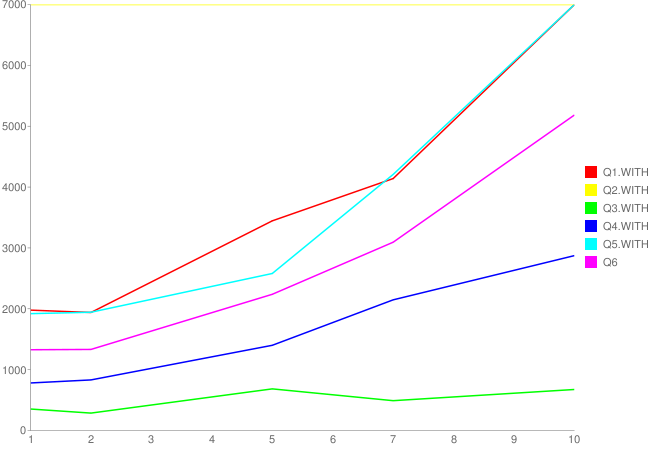
\includegraphics[width=0.85\textwidth]{figures/benchmark-WITH-2000.png}
	\caption{Durchschnittliche Response-Time bei einer Wartezeit von 2 Sekunden unter Verwendung von \texttt{WITH}-Tables}
 \end{figure}
 
 Bei noch h�herer Server-Belastung skalieren Q3 und Q5 mit \texttt{WITH}-Tables besser als ohne.
 
 \newpage
 \subsection{Q7 mit 2 Sekunden Wartezeit}
 
 Das Benchmark-Ergebnis von Q7 mit einer Wartezeit von zwei Sekunden einmal mit tempor�ren Tabellen und einmal mit \texttt{WITH}-Tables:
 
 \begin{figure}[htbp]
	\centering
		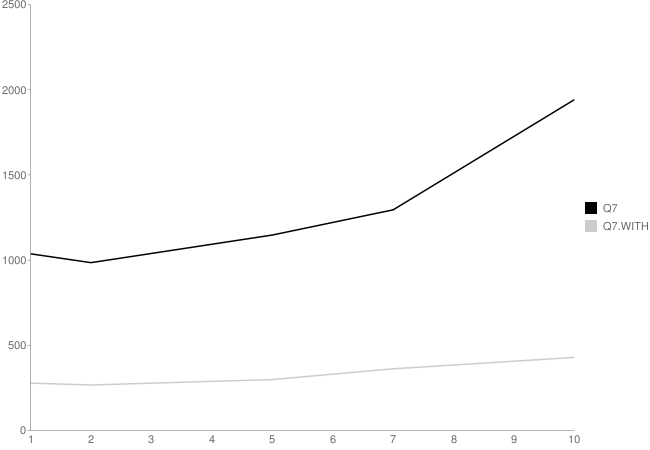
\includegraphics[width=0.85\textwidth]{figures/benchmark-Q7-2000.png}
	\caption{Durchschnittliche Response-Time bei einer Wartezeit von 2 Sekunden}
 \end{figure}

 Auch Q7 ist mit \texttt{WITH}-Tables performanter als ohne.
